\section{总体分析与总技术路线图}

\subsection{总体分析}

本题的核心是一个在复杂地形与通信约束下，运输无人机、中继无人机与能源资源多类要素的协同优化问题，四个子问题呈递进关系，公共物理规则、单位与对象编号保持一致。

\textbf{问题一}是能力评估与组批问题。每个架次为单服务区直接往返，故各服务区相互独立，问题可分解为“单点往返最大安全载荷计算”与“货箱装箱组批”两个层次。前者由地形净空（巡航海拔）、等效航程模型和爬升附加能耗共同决定，可用二分法精确求解；后者是典型的一维装箱（bin packing）问题\cite{martello1990knapsack}，货箱不可拆分且需同时满足质量、体积与能量余量约束。

\textbf{问题二}是带资源约束的多机型车辆路径问题（VRP）的推广\cite{dorling2017vehicle}。相比经典 VRP，其难点在于：载荷随投送过程递减使得航段能耗非线性；共享电池按机型分池且需两阶段充电周转；医疗与首批物资带硬时限。由于规模较大且约束耦合，采用“构造启发式＋离散事件调度”的两阶段求解策略，并用对比实验刻画指标间的权衡。

\textbf{问题三}在问题二的基础上叠加通信约束，是运输—中继联合调度问题。通信状态由视线遮挡（地形）与双向链路预算共同判定\cite{itu2024p525,zeng2016wireless}，需对运输无人机轨迹逐时刻采样判定直连/中继/中断三种状态；中继悬停位置与时段则构成一个带时间窗的几何覆盖问题，可用“候选点网格＋集合覆盖”求解。

\textbf{问题四}是任务分区与资源配置问题。在保持问题三调度关系不变的前提下，将服务区划分为若干任务组，本质是对“多服务区架次”所约束的服务区进行聚类，并在组间不可调配资源的条件下核算各组峰值资源需求，进而比较不同分区方式的资源规模、冗余与缺口。

四个问题间的数据继承关系为：问题一的组批能力与能耗模型为问题二提供基础；问题二的运输调度方案为问题三的通信分析提供运输轨迹与时段；问题三的联合调度方案为问题四的分区提供待划分的任务单元。据此，本文首先统一建立公共物理模型，再逐问递进求解：问题一给出的最大安全载荷与组批结论构成问题二装箱时的容量输入，问题二得到的运输架次及其时段是问题三逐时刻判定通信状态的直接对象，问题三的运输—中继联合调度方案又构成问题四划分任务组时的待绑定单元。上述路线汇总于下页的总体技术路线图。

% 参照竞赛优秀论文的通行画法：整页竖排、纯黑白、每条带对应一个子问题，
% 纵向五带（公共物理模型＋四问）× 横向四栏（阶段），节标题即图题。
% 三点务必保留：① 不加 \caption（否则白占一个图号，且与节标题重复）；
% ② 用 \clearpage + 非浮动排版的精确落版，改用 [p] 浮动体会被推迟若干页；
% ③ 宽度取 0.97\textwidth——按 0.97 计高 621pt，加节标题 40pt 后余量 27pt，
%    取满 \textwidth 则只剩 8pt 余量，字号或行距稍变即溢出到次页。
\clearpage
\subsection{总技术路线图}

\begin{center}
	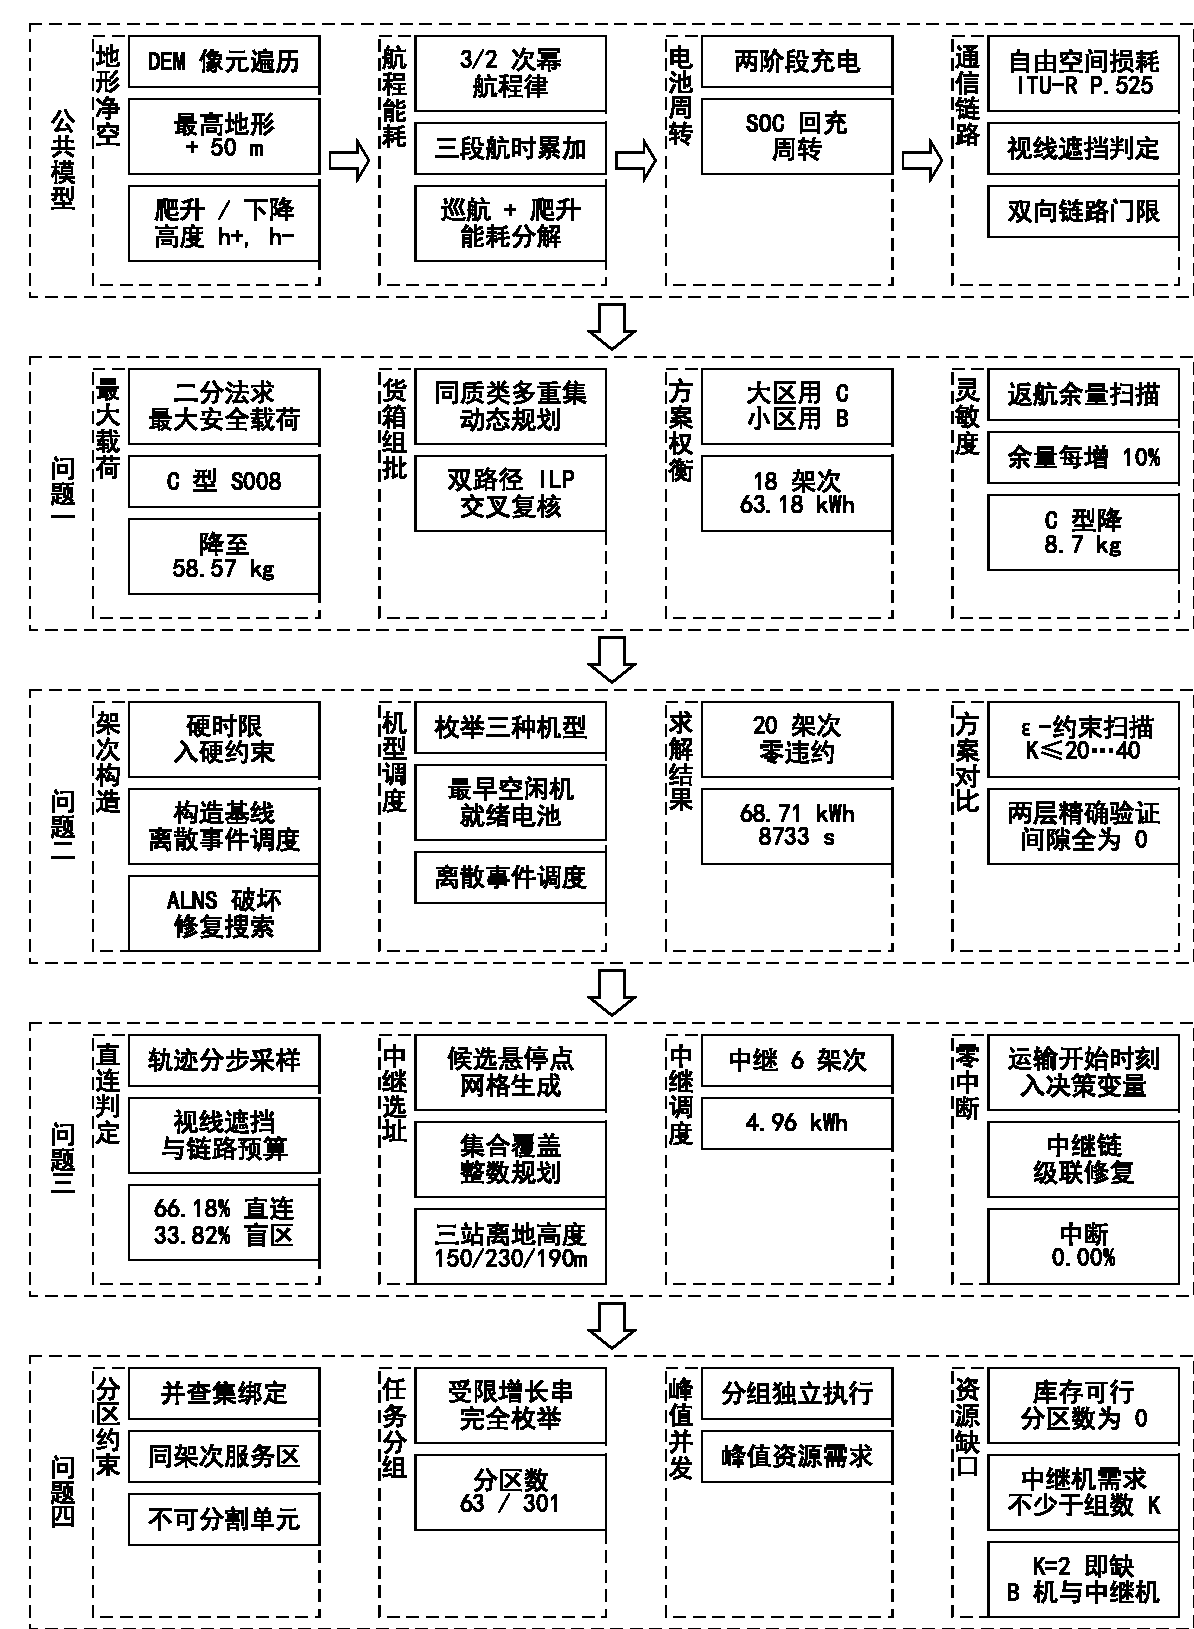
\includegraphics[width=0.97\textwidth]{figures/fig_roadmap.pdf}
\end{center}
